\documentclass[conference]{IEEEtran}
\IEEEoverridecommandlockouts
% The preceding line is only needed to identify funding in the first footnote. If that is unneeded, please comment it out.
\usepackage{cite}
\usepackage{amsmath,amssymb,amsfonts}
\usepackage{algorithmic}
\usepackage{graphicx}
\usepackage{textcomp}
\usepackage{xcolor}
\usepackage{natbib}
\usepackage{graphicx}

\usepackage{todonotes}
\newcommand{\cit}{\todo[tickmarkheight=0.2cm]{cit}}

\def\BibTeX{{\rm B\kern-.05em{\sc i\kern-.025em b}\kern-.08em
    T\kern-.1667em\lower.7ex\hbox{E}\kern-.125emX}}
\begin{document}

\title{Can AI be explained? \\
    The XAI approach and its limits}

\author{\IEEEauthorblockN{Alvise de' Faveri Tron}
    \IEEEauthorblockA{\textit{Politecnico di Milano} \\
        alvise.defaveri@mail.polimi.it}
}

\maketitle

\begin{abstract}
    \todo[inline]{TODO}
\end{abstract}

%-----------------------------------------------------------------%
\section{Introduction}
\label{sec:intro}

Artificial Intelligence (AI) has come a long way since its birth in the late '50s.
\cit In the last decade, in particular, we have seen amazing
improvements in this field.

It has become increasingly pervasive, with successful applications in the
medical, legal, law enforcement, financial and automotive fields. \cit This success
is undoubtedly shaping today's and tomorrow's society, since many tasks that
were exclusively carried out by humans can now be handled in an autonomous way.

% by AI systems: some go as far as calling the current period a "fourth
% industrial revolution" \note{cit} caused by AI or talk about the "AI
% singularity" \note{cit} referring to the fact that nothing like this has been
% seen before in human history.

However, AI as a technology has just started its journey: there are currently
many limitations and shortcomings that emerge when observing real-world implementations. One issue in particular has been found to be
recurring and problematic, since it deeply undermines the trust and reliability
of this technology: the fact that we don't understand enough about it. \todo[inline]{troppo drammatico}

Machine Learning and Neural Networks in particular, which are the most common
and performing AI algorithms today \cit , are difficult for humans to debug.
Introspection tooling around this kind of technology is currently insufficient,
and yet essential. We need to devise new methods to validate AI algorithms, find
weaknesses and possibly correct them with a human-in-the-loop approach.

Explainable Artificial Intelligence (XAI \cit) is a relatively new field of AI that aims at addressing this
problem. Many interesting results have been achieved in this field, and many
more are expected in the next years, but there are still some fundamental
issues, which are common to many modern AI algorithms but are particularly
evident in Machine Learning, that have yet to be addressed in a general and
consistent way.

The goal of this paper is to identify and discuss some of such inherent issues,
analyze their root causes, and argue that the current XAI approach
generally fails to address them.

\subsection{Structure of this paper}
\label{sec:structure}

Before we discuss the problems of XAI, we need to give some context about what
XAI is trying to achieve and for which purpose.

In Section~\ref{sec:problem} we will start by looking at some examples  that we consider relevant to understand the XAI problem in detail.

In Section~\ref{sec:xai} we give a more specific definition of XAI and a general
overview of the solutions that are being developed in this framework.

Finally Section~\ref{sec:missing} contains a reflection on what is not
being considered by XAI, in particular: the causality vs correlation problem,
the problem of measuring the quality of explanations, the biases introduced by
an explanation, and the problem of measuring the fidelity of an explanation.

\todo[inline] {narrow down the claims?}
\todo[inline] {alt version: \textit{contains a reflection on what are the dimensions that XAI fails to explore, in particular the evaluation of an explanation.}}

%-----------------------------------------------------------------%
\section{Background}
\label{sec:background}

\subsection{Machine Learning}
\label{sec:ml}

One very popular and effective technique in AI is Machine Learning, and in
particular Supervised Learning \cit. This approach generally consists in
\textit{training} an algorithm by giving it as input a large number of instances
of a given problem and letting it figure out on its own the best way to model it. The
strength of this technique is that no previous knowledge of the model of the
problem is needed, nor it can be enforced generally, and this is exactly
where this technology gets an edge over more traditional computer science
approaches.

\subsection{Artificial Neural Networks}
\label{sec:nn}

A particular way of implementing a Machine Learning algorithm is through Artificial Neural Networks (ANN), which are an extremely powerful tool that is being employed for many complex problems nowadays, from computer vision to data analysis, showing unprecedented results. The idea is to have a fixed structure made of interconnected \textit{neurons}, whose connections, called \textit{weights}, are modified in the learning phase by the learning algorithm.

\subsection{Programming AI}
\label{sec:aiprog}

In the aforementioned techniques, the programmer gets to decide only one aspect of the solution, which is the number of layers, neurons and activation functions in the case of Neural Networks, but is not in control of the whole output of the algorithm, which is \textit{learned} using the data it is fed with.

Measuring the quality of the dataset and eliminating possible biases from it, preventing the algorithm form learning a biased or unfair model, is a huge matter of discussion in the field \cit, that goes beyond the scope of this paper.

However, what we want to highlight here is that the problem of not having a total control over the algorithm output is not an exclusive feature of Neural Networks, but is a common trait of AI algorithms in general. While a strict definition of what AI is and isn't is still a matter of discussion \cit, we can observe that many AI algorithms, if not all of them, are in fact \textit{meta-}algorithms, i.e. algorithms that define how the solution space of a given family of problems should be \textit{explored}, not how to find the solution itself \cit. This aspect is crucial to understand some of the peculiarities of the explainability problem in AI, which is not present in traditional computer programming, at least not in the same form.

%-----------------------------------------------------------------%
\section{The Problem}
\label{sec:problem}

\subsection{AI failures}
\label{sec:aifails}

The observation of how AI systems behave in various fields has shown
us one interesting fact: when these systems break, they tend to break hard. A single
misprediction made by a Machine Learning algorithm, in particular, can cast a shade on the correctness of the whole model
itself, on the data it has been trained on or on its design. There's rarely such
thing as ''fixing one line of code'' on deep neural networks that have been
trained on millions of data points: once its trained, you either add more data
or start again from scratch, which can be a very high price to pay in terms of
time and computational power.

\todo[inline]{Esempi concreti invece che claim astratti?}

Moreover, these kind of errors are generally difficult to predict in advance: an
AI algorithm can perform very well on a high number of inputs, but have a weak
point that is only discovered way after the AI has been deployed. The same people that design and train the algorithm have generally little
knowledge about what model the network is going to produce at the end, and when
it does the only way of verifying its correctness is black box testing, for
which the input space is generally huge.

All these considerations have encouraged the AI industry and the governments to
tackle the problem of understanding an AI model and "opening" the black box.

\subsection{A toy example}
\label{sec:example}

As an example of the problem of explaining an AI system, a representation of a Neural Network's conceptual structure is depicted in Figure~\ref{fig:nn}.

\begin{figure}[ht!] \centering 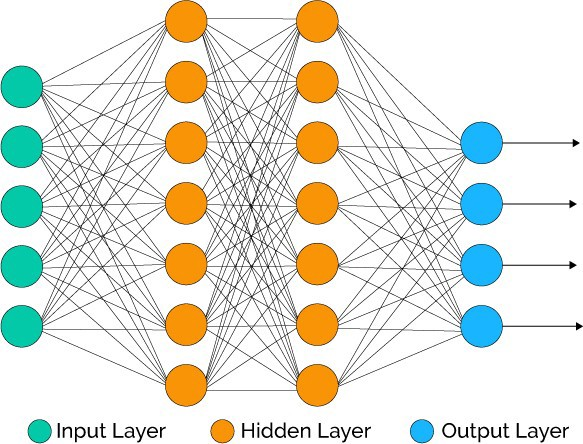
\includegraphics[width=0.8
        \linewidth]{images/nn}
    \caption{Simple representation of an Artificial Neural Network} \label{fig:nn} \end{figure}

The graphical representation is useful for understanding the general architecture of a Neural Network, but it doesn't really tell us anything about how the Neural Network actually works, i.e. what is the relationship between a certain input and a certain output.

We could give a more precise representation of this dependency in Figure~\ref{fig:mathnn}, which explicitly defines the mathematical relationship between the input and the output. Without going into the details of the mathematical formula, we can see how we would still have a hard time understanding what a Neural Network does if we were to adopt this representation.

\begin{figure}[ht!] \centering 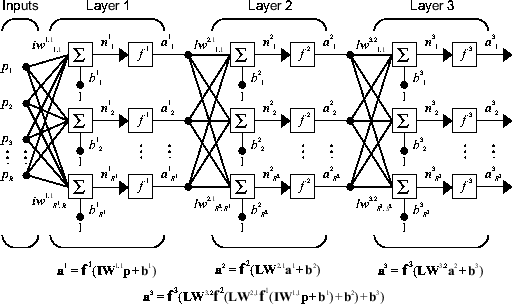
\includegraphics[width=0.9\linewidth]{images/nmodel}
    \caption{Mathematical equivalent representation} \label{fig:mathnn} \end{figure}

On the other hand, Figure~\ref{fig:dectree} represents a \textit{Decision Tree}, another family of AI algorithms. While on one hand we can easily agree that this type of representation is more intelligible and tells us more about how the AI algorithm constructed its model, we have to deal with the fact that Neural Networks generally perform better than Decision Trees.

\begin{figure}[ht!] \centering 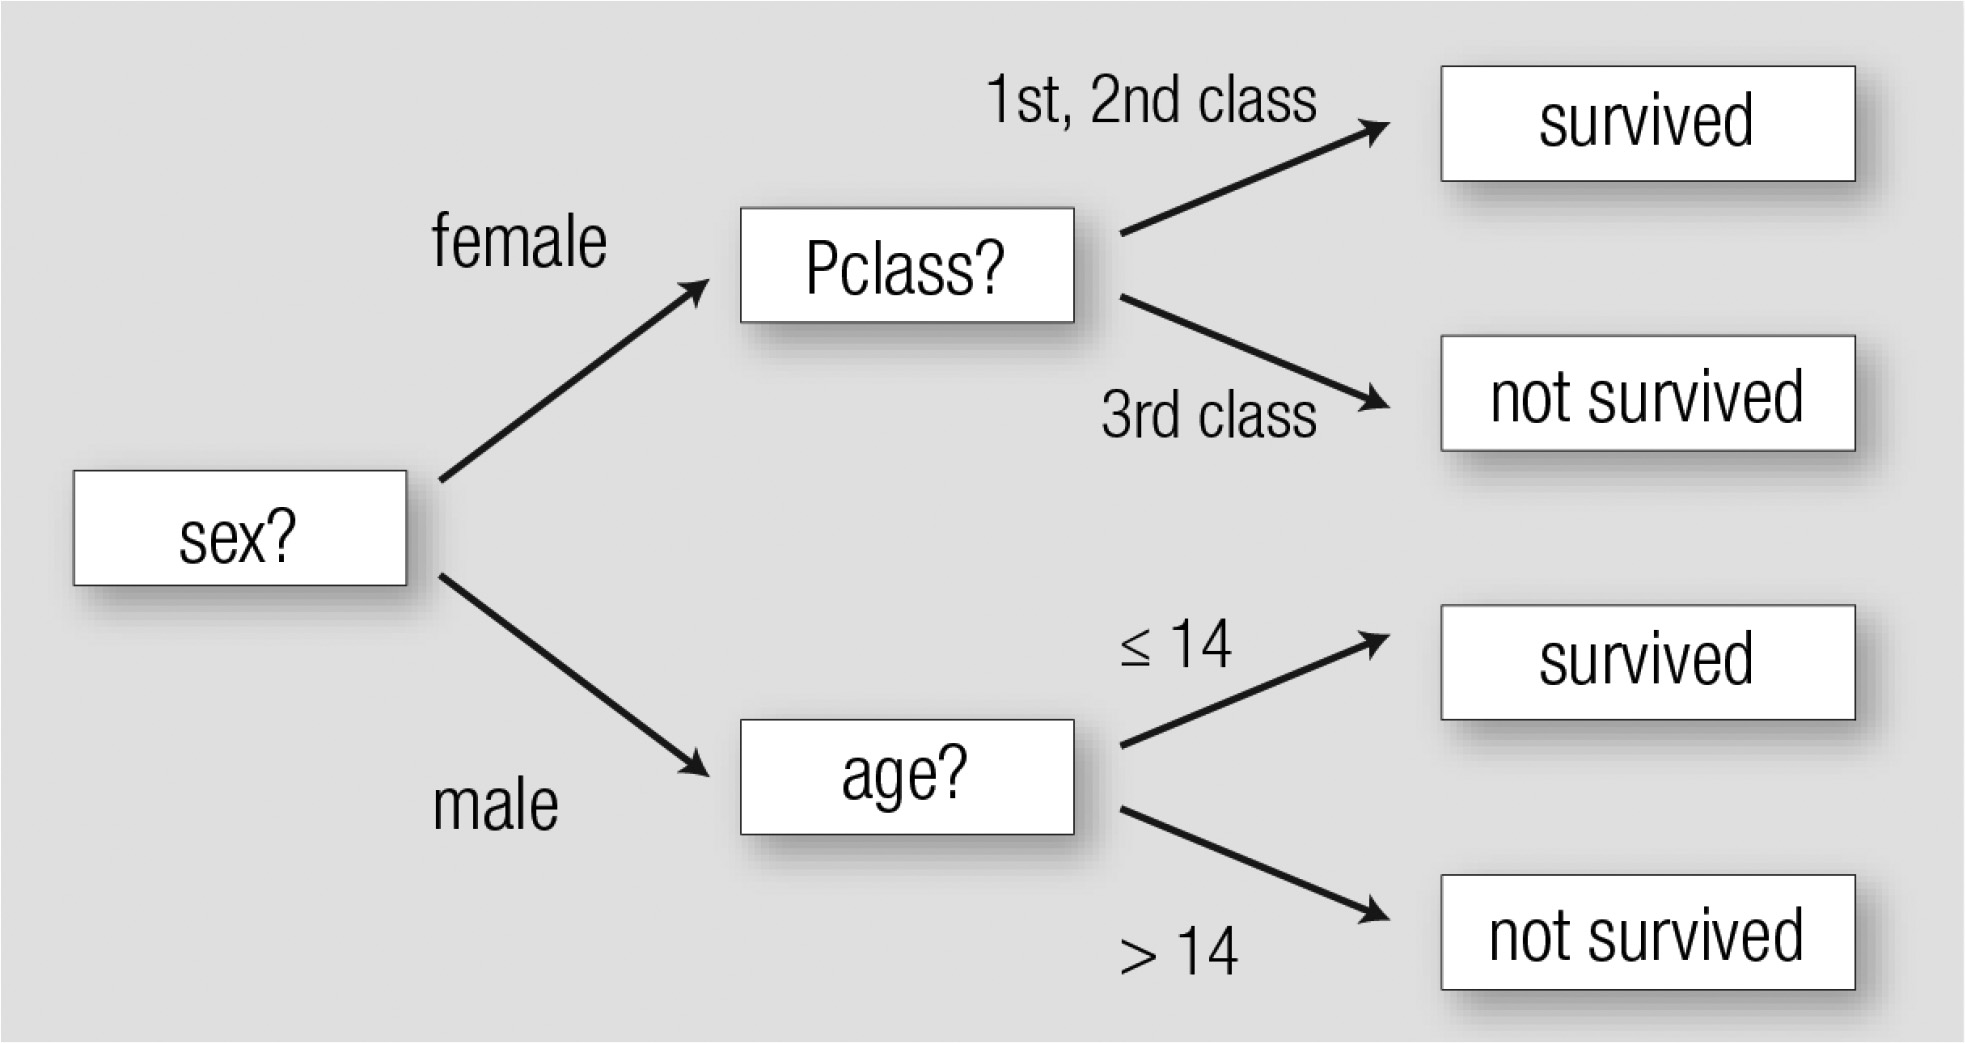
\includegraphics[width=0.9\linewidth]{images/dectree}
    \caption{A simple Decision Tree} \label{fig:dectree} \end{figure}

This simple example shows how the solution space to the explainability problem has multiple dimensions, constraints and trade-offs that have to be taken into account.

%-----------------------------------------------------------------%
\section{The XAI approach}
\label{sec:xai}

\subsection{The goal}

Explainable AI is a concept that was recently formalized in a call for research made by DARPA \cit, the same agency where the word "Artificial
Intelligence" was born in the first place \cit. It is meant to be describe a new set
of Artificial Intelligence systems which are designed to be easier to understand
by humans. In particular, the goals of XAI is making artificial intelligence
more:

\begin{itemize}
    \item \textbf{Easy to debug} and correct
    \item \textbf{Predictable}, so that companies and governments adopting this technology can be aware of the possible weaknesses of a their models, and can be held responsible when using bad algorithms
    \item \textbf{Trustful} for operators and end-users of this technology
\end{itemize}

Figure~\ref{fig:xai} is taken from the DARPA presentation on XAI and describes the kind of goals for which it has been proposed.


\begin{figure}[h!] \centering 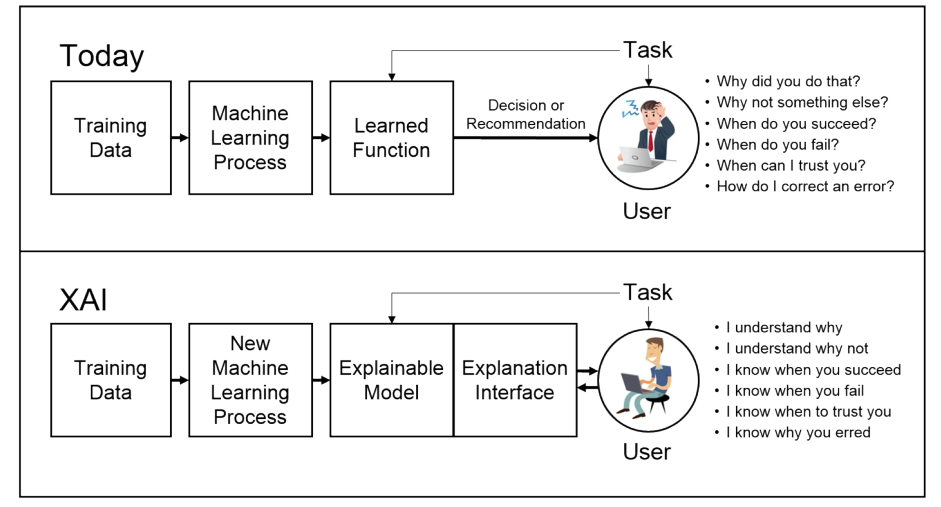
\includegraphics[width=\linewidth]{images/xai.png}
    \caption{The XAI concept \todo[inline]{cit} } \label{fig:xai} \end{figure}

The creation of XAI requires the join effort in a variety of research fields, from Computer Science to Cognitive
Psychology, and there is still a lot of work to do. Nevertheless already many papers have been submitted on the subject \cit, indicating a growing interest of the research community towards this subject.

\subsection{A multitude of approaches}
\label{sec:dimensions}

An overview of the literature on XAI reveals how solutions presented under the name of XAI may vary greatly in the aspects they consider when presenting their solution. To have an idea of how how varied the solution space is, we might ask ourselves the following questions when analyzing XAI proposals:

\

\textbf{Explainable to whom?} The concept of \textit{user} of an AI system is not always well defined, nor is the concept of user of an explanation. This might include:

\begin{itemize}
    \item The \textbf{developer} of the AI system, as he is only partially in control of what the algorithm does (refer to Section~\ref{sec:aiprog})
    \item The \textbf{operator} of an AI system: many AI algorithms nowadays are being used as an input for a human to make decisions on a certain subject
    \item The \textbf{end user} which is affected by the decision of an AI
\end{itemize}

\

\textbf{Explainable for which purpose?} Different users have different needs, that can partially overlap, when it comes to AI explanation. More in general, whether a certain representation can be considered and explanation or not depends in some sense on what the explanation is being used for. In the case of XAI, some common purposes are:

\begin{itemize}
    \item \textbf{Debugging}: finding errors or underperforming portions of the system
    \item \textbf{Human-in-the-loop}: creating systems where human and AI decisions can co-exist and influence each other
    \item \textbf{Validation}: understanding if a certain model is good enough to be deployed for a certain tasks, where it fails and what happens when it fails
    \item \textbf{Appeal AI decisions}: giving the right to users and citizens that are affected by Ai decisions to know, understand and possibly appeal decisions that are automated with Ai systems
\end{itemize}

This last goal is not explicitly listed in the original scope of XAI goals, but has gained traction recently with the publication of \textit{right for an explanation} law in EU. \cit

\

\textbf{Explainable in which sense?}

One of the main problems of XAI is that there is no unique way of defining how should an explanation be evaluated. Some \cit go even as far as considering the term \textit{interpretabilty} as ill-defined, since there is no consensus on what the definition should be. While we will explore this concept in depth in Section~\ref{sec:missing}, here we propose a classification of some of the dimensions upon which an explanation can be evaluated:

\begin{itemize}
    \item \textbf{Complexity}: how many elements are there in the explanation?
    \item \textbf{Clearness}: how cognitively hard is the explanation? How difficult is it to understand the correspondence between the elements of the explanation and the information we are trying to gain?
    \item \textbf{Informativeness}: how much information, weighted of how meaningful they are, can be extracted by the explanation? E.g. does the information given by the explanation significantly modifies the level of uncertainty that the user has about the Ai behavior?
    \item \textbf{Fidelity}: how closely does the explanation represent the internal functioning of the system? Do single elements of the explanation have a correspondence to well-defined set of elements in the original structure? How much information is lost when passing from the initial structure to the explanation?
\end{itemize}

\subsection{Current Solutions}
\label{sec:solutions}

Given the highly experimental nature of this topic, many different solutions have been proposed by various papers in the framework of XAI, which vary greatly in intended use, goal and adopted approach. Giannotti et al. \cit contains a details and exhaustive description and classification of the existing XAI solutions and their respective strengths and weaknesses. With no aim of being comprehensive or in any way technically precise, here we give a more abstract classification of popular XAI solutions, based their general approach to the problem.

XAI approaches might be classified as:

\begin{enumerate}
    \item \textbf{Visualization}: improving the understanding of a model using a better way to visualize its internals. One popular application of this approach is computer vision, where features of the learned model might be mapped onto the input image. \cit
    \item \textbf{Simplification}: similarly to the idea explained in Section~\ref{sec:example}, this approach consists in trying to adopt simpler models or simplify already existing models to just a set of important features. \cit
    \item \textbf{Reverse Engineering}: once a model has been produced by an AI, one explanation technique is to try and understand the dependencies between inputs and outputs by trying to find which output change is triggered by a given input change. Most of the times this means, in practice, creating a behavioral model of the algorithm which is parallel to the algorithm itself, and has no immediate correlation with the algorithm's internal structure.
    \item \textbf{Explain by Example}: a nice information to have when trying to understand an AI model, especially in the case of classifiers, is an example, or a \textit{prototype}, of how the AI thinks that a typical member of a given class should appear. This can be realized in many ways, for example by attaching to a classification output a set of minimal changes to the input that would cause the output to be modified, or specify a partially filled object for each class.
\end{enumerate}

\todo[inline]{Immagini esemplificative}

\todo[inline]{Si può integrare con una classificazione più classica delle tecniche (internal vs external ecc)}



%-----------------------------------------------------------------%
\section{What's missing?}
\label{sec:missing}



\begin{itemize}
    \item Correlation vs causality
    \item Double Standard human vs Machine
    \item Evaluating an explanation
\end{itemize}

Ma come valutare le soluzioni? Basta la complessità?

The problem is that there is a lack of a formal definition of how an explanation
should be measured. This is not a trivial point, since it is very difficult to
quantitatively measure the goodness of any explanation. Many papers refer to
complexity but this is not enough.

\subsection{Why is there an explainability problem in the first place?}

\begin{itemize}
    \item causality vs correlation
    \item previous categories
    \item having a goal -> the decision means that I have to do something in
          practice, and that thing has an ethical an practical impact
\end{itemize}


\subsection{Can they be measured separately?}

\begin{itemize}
    \item fidelity vs complexity
    \item fidelity vs clearness
    \item quality vs performance
\end{itemize}

%-----------------------------------------------------------------%

\section{Conclusions}
\label{sec:conclusions}

In conclusion, the main problem of XAI is that there is no single definition of
what an explanation is, it depends on the purpose and on the user of the AI
system.

For this reason, these should be considered different problems, at least the
debugging problem vs the right of explanation problem: they are not correlated
and saying that one solves the other poses some threats on the quality of the
result itself.

``I always thought something was fundamentally wrong with the universe''
% \citep{adams1995hitchhiker}

\bibliographystyle{plain}
\bibliography{references}
\end{document}
